\section{Hybrid (MPI and OMP)}\label{sec:hybrid}
\subsection{Implementation}
MPI and OMP interact seamlessly when put together, making it easy to combine
our MPI implementation and the origin OMP implementation. Given a fixed number
of MPI ranks, $r$, and $p$ available threads then each MPI rank will have
access to $p/r$ threads which can be used in OMP parallel sections of code.
This can mean we do not take full advantage of all threads available to us if
$p$ is not divisible by $r$. We implemented a hybrid version (by combining our
MPI implementation and the OMP parts of the original implementation) in
\texttt{path-mpi-omp.c}

\subsection{Performance}
To study the performance of our hybrid code we did strong scaling studies for a
large range of n and used baselines of our hybride code with 1 MPI rank (Figure
3), our MPI code with 1 MPI rank (Figure 4), and the given OMP code with 24 OMP
threads available (Figure 5).

\begin{figure}[h]
  \centering
  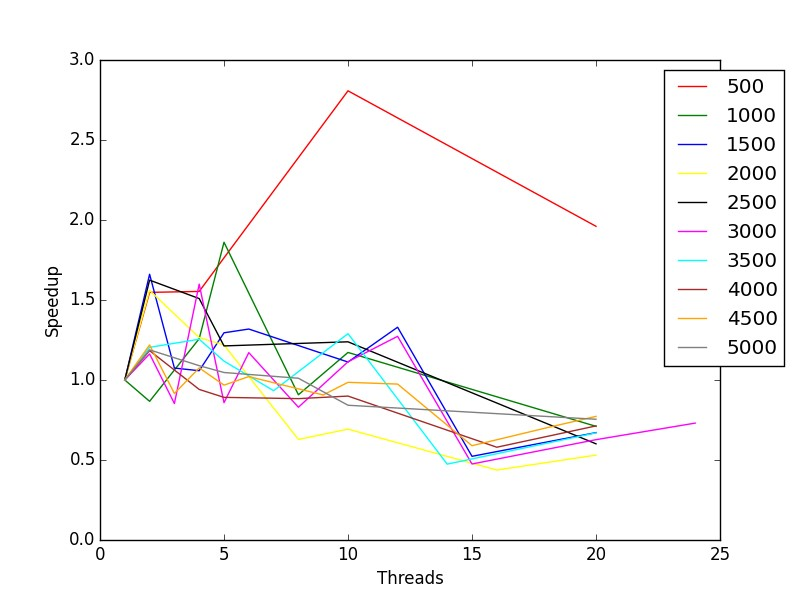
\includegraphics[width=0.63\textwidth] {plots/3}
  \caption{%
    Strong scaling speedup of our Hybrid code as number of MPI ranks increase
    (changing the number of available OMP threads to each rank) increase.
    Baseline for calculating speedup is Hybrid with 1 MPI rank.
  }
  \label{aload0}
\end{figure}
\begin{figure}[h]
  \centering
  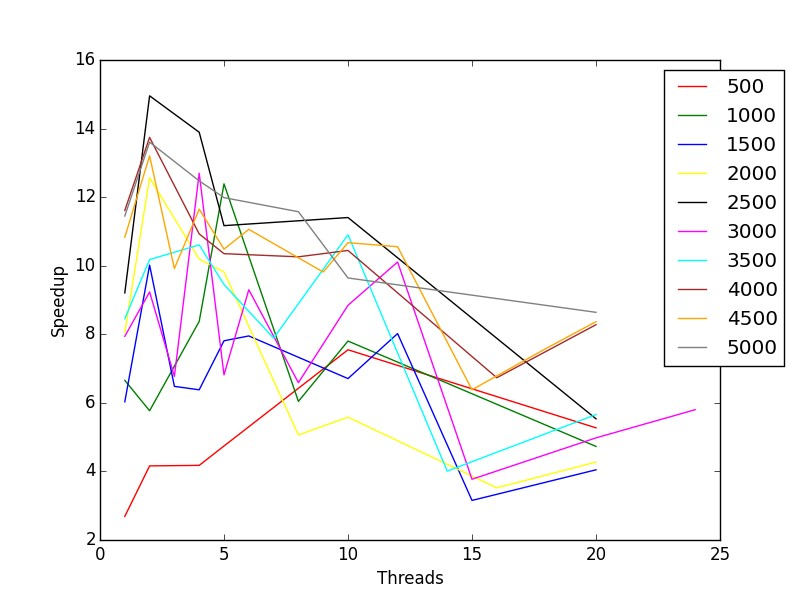
\includegraphics[width=0.63\textwidth] {plots/4}
  \caption{%
    Strong scaling speedup of our Hybrid code as number of MPI ranks increase
    (changing the number of available OMP threads to each rank) increase.
    Baseline for calculating speedup is MPI with 1 MPI rank (thus 1 thread
    total).
  }
  \label{aload1}
\end{figure}

\begin{figure}[h]
  \centering
  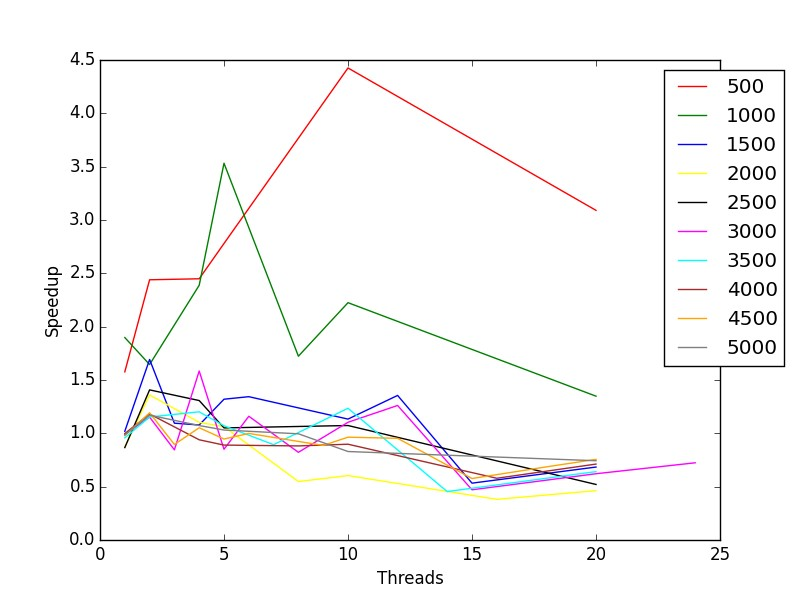
\includegraphics[width=0.65\textwidth]{plots/5}
  \caption{%
    Strong scaling speedup of our Hybrid code as number of MPI ranks increase
    (changing the number of available OMP threads to each rank) increase.
    Baseline for calculating speedup is OMP code with 24 threads.
  }
\end{figure}

In Figure 3 we can see that increasing the number of MPI ranks (which in turn
decreases the number of OMP threads per rank) has mixed speedup for most n.
When the number of MPI ranks is less than 10 we often have speedup larger than
1, but as we go beyond 10 and 12 speedup drops off. This is because of
increased MPI overhead across 2 chips and the hybrid codes inability to take
advantage of all possible threads when there are more than 12 MPI ranks.

In Figure 4 our hybrid code gets large speedup over the (serial) MPI code (1
rank) for all n. This is because mixing MPI and OMP allows the code to take
advantage of more threads than is possible with MPI alone as OMP will take up
remaining threads which aren¡¯t allocated to MPI ranks.

In Figure 5 our hybrid code sometimes manages to get speedup of over 1 as
compared to  the OMP code. This indicates that mixing MPI and OMP can lead to
better thread utilization than using OMP alone.
